\chapter{Analog Measurement} \labchap{analog_measurement}
In electronics, there are two different types of signals: digital and analog.
Digital signals are either a ``high'' voltage, or a ``low'' voltage, representing either a logical 0 or logical 1.
These signals are great for threshold measurements such as ``is there a cart present at the start of the ride, yes or no?'', but cannot express a range of values.
Conversely, analog signals are better suited to expressing real-world values that naturally vary from a minimum to a maximum and can be any value in between.
Thus, analog signals are prevalent for devices that measure ``real'' things such as speed, acceleration, rotation rates, barometric pressures, etc.

\begin{figure}[h!]
    \caption[Analog versus digital waveforms]{A digital square wave (top) versus an analog sinusoidal wave (bottom).
    Courtesy of SparkFun \cite{SparkFun:AnalogDigital}}
    \labfig{analog_vs_digital}
    \centering
    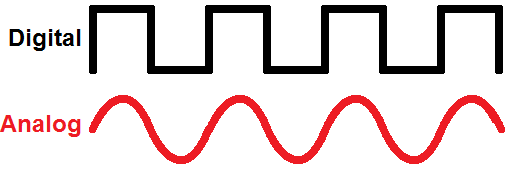
\includegraphics[width=0.5\textwidth]{appendices/analog_measurement/analog_vs_digital.png}
\end{figure}

Most analog sensors are resistive types where their electrical resistance changes to scale with a real-world measurement range.
Ohm's Law defines the relation between voltage, ($V$) resistance ($R$), and current ($I$) as $V=IR$.
Therefore, if we can measure the voltage drop across a resistive sensor and correlate it with a manufacturer-provided equation or table, we can quantify a real-world phenomenon.
The resistance is best measured using a Wheatstone Bridge and an amplifier which can generate a voltage that is directly proportional to the change in resistance, $\Delta R$

\section{Analog to Digital Conversion} \labsec{analog_to_digital_conversion}
Now that we can get a sensor reading as an analog (changing) voltage, we need to find a way to translate it into a useful form.
Decades ago, the analog voltage from a sensor was plotted onto a chart with respect to time and an analyst could run the conversion point by point.
In a real-world experiment, it would be very difficult to deploy a large plotter to capture field data.
We also want to work smarter and not harder, so we want a computer to perform the analysis for us. 
What can we do?
Since we live in the digital age, we can convert the analog signal to a digital one and then we can store it on a digital media device such as an SD card then load it directly into a computer program like Excel to analyze it.

This process is done with an analog to digital converter circuit or ADC. 
The ADC samples an analog waveform at a given frequency and places the voltage level into bins for each measurement.
There are $2^N$ bins in an ADC depending on its resolution, $N$.
For each measurement, the ADC will also encode the voltage reading as a binary number and save it to a register.

This encoded binary number is expressed as ``counts'' which can be read by a microcontroller or other digital system.
The number of counts recorded can be converted back to a voltage value at any time using the equation below.
However, this conversion will lose some of the original precision of the analog signal, depending on the resolution of the ADC.
A higher resolution will mean a more precise reading.

\begin{equation*}
    V = V_{\text{s}} \frac{\text{counts}}{2^N}
\end{equation*}

\begin{figure}[h!]
    \caption[Analog to digital converter waveform]{A 3-bit ADC waveform converting an analog sinusoidal voltage wave (red) of period, $T$, to a digital representation (black).
    Each ADC bin is shown by a blue dashed line.}
    \labfig{adc_wave}
    \centering
    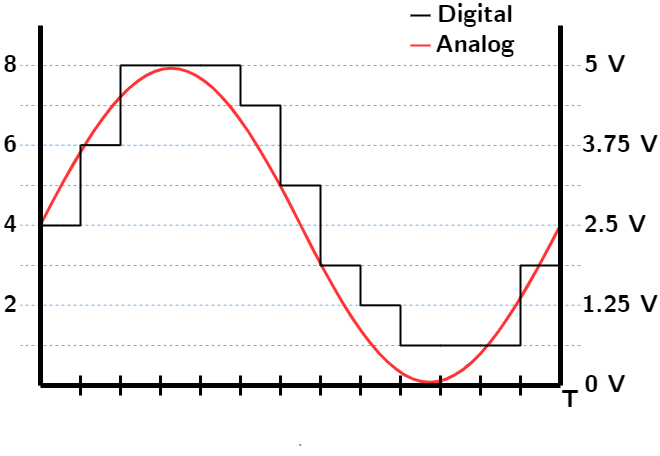
\includegraphics[height=2.5in]{appendices/analog_measurement/adc_wave.png}
\end{figure}

\begin{figure}
    \centering
    \begin{fitbox}[frametitle=Aside: Registers]
        Digital values are stored in memory as 1's and 0's.
        Each bit of memory can be stored in a contiguous piece called a ``register''.
        A digital system can access registers of memory to grab values and perform calculations on them.
        For example, an 8-bit ADC will store the encoding of an input signal in an 8-bit register.
        A microcontroller can then read this value from the ADC and convert it to a real-world value, or save it to non-volatile memory for logging.

        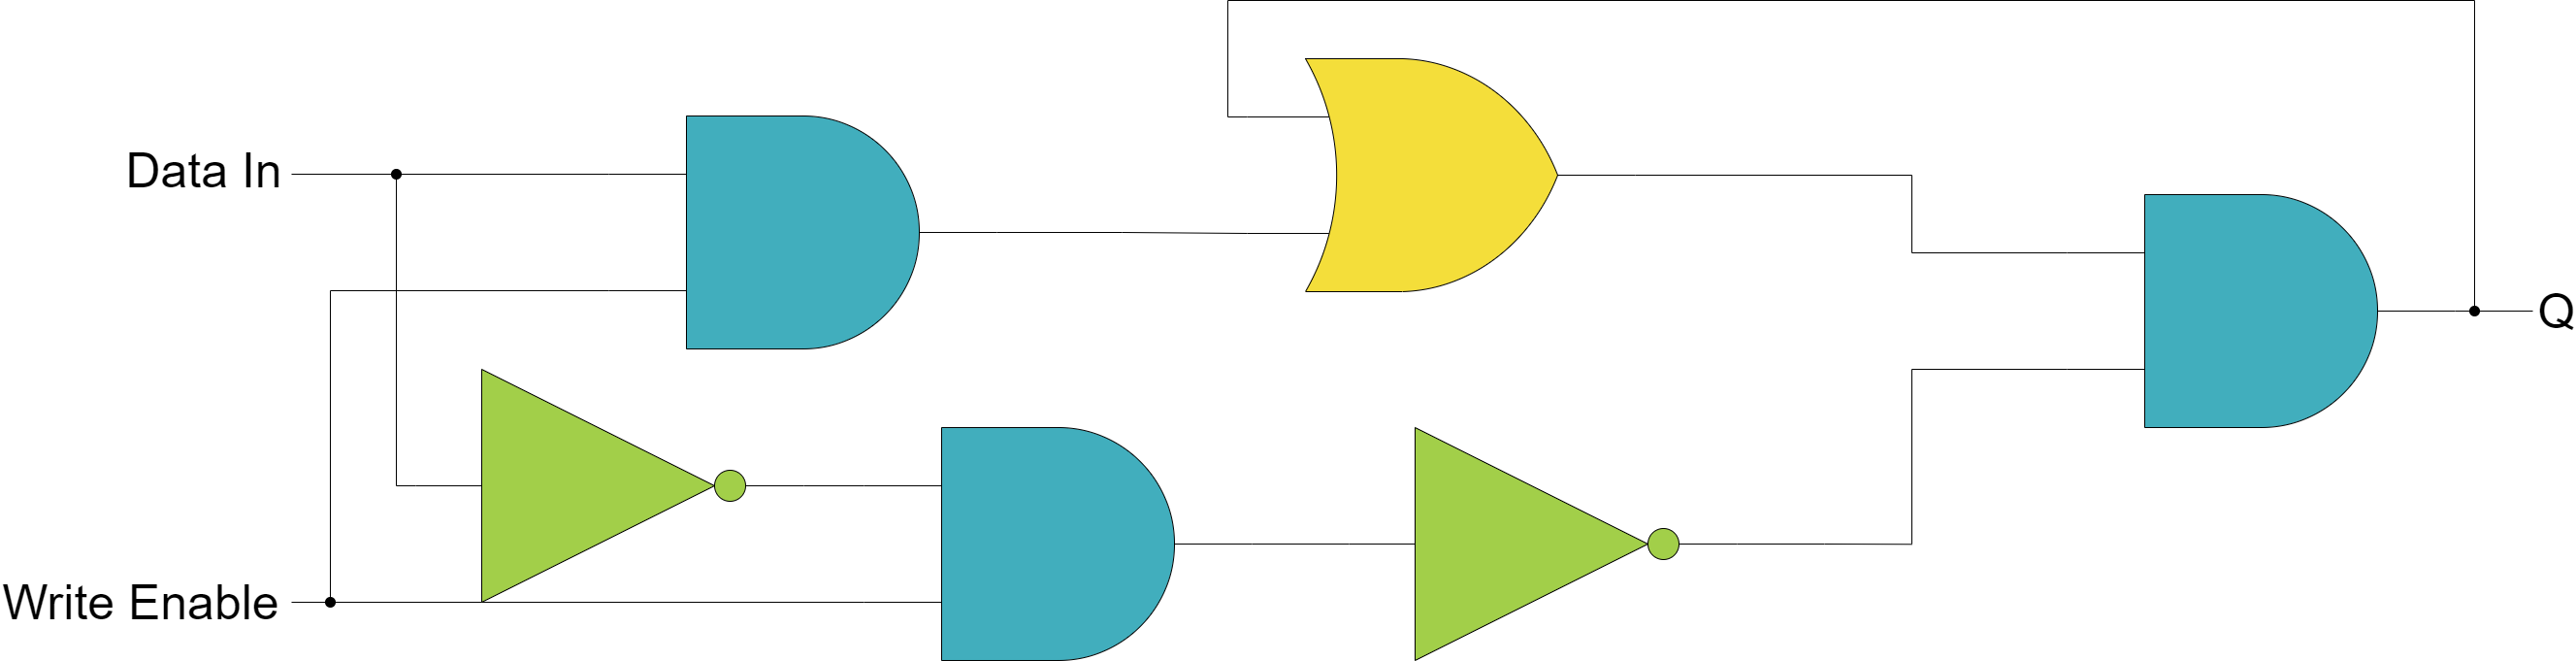
\includegraphics[width=\textwidth]{appendices/analog_measurement/gated_latch.png}
        \caption{A gated latch circuit used to store 1 bit of memory.}
    \end{fitbox}
\end{figure}